\section{Vergleich von populären Enterprise Messaging Services}

Zwei der populärsten Messaging-Systeme, die in der Softwareentwicklung weit verbreitet sind, sind \emph{Apache Kafka} und \emph{RabbitMQ}. Beide Systeme bieten leistungsstarke Funktionen für das Messaging und adressieren unterschiedliche Anwendungsfälle und Anforderungen. In diesem Kapitel wird ein detaillierter Vergleich zwischen diesen Messaging-Systemen durchgeführt. Zusätzlich wird ihre Architektur, Funktionalitäten, Leistungsmerkmale, Einsatzszenarien und weitere relevante Aspekte analysiert, um Entwicklern und Architekten dabei zu helfen, die richtige Entscheidung für ihr Messaging-System zu treffen. Dabei werden sowohl die Stärken als auch die Schwächen dieser beiden Systeme beleuchtet, um einen umfassenden Einblick in ihre Unterschiede und Gemeinsamkeiten zu bieten.

\subsection{Apache Kafka}
\label{kakfaExplained}

Kafka ist ein hoch skalierbares und verteiltes Messaging System, welches bekannt für die Fähigkeit große Datendurchsatzraten erreichen zu können ist. Dieses System wird in der Scalar Programmiersprache geschrieben und hat eine sehr aktive Community, die das open-source Projekt ständig um Funktionen erweitert. Apache Kafka wird auch als Streaming-Plattform bezeichnet, da es die Anforderungen an Stream-Processing genügen kann. Stream-Processing ist die Datenverarbeitung an einen Fluss von Daten, also eine unendliche Serie an Daten. Das \emph{Messaging System} von Apache ist für diesen Anwendungsfall gut geeignet, da es in der Lage ist, die benötigten Durchsatzraten zu erreichen und eine Reihe an Stream-Processing Funktionalitäten besitzt, wie zum Beispiel \emph{Kafka Streams} oder \emph{KSQL}. Außerdem verfügt Apache Kafka über \emph{Connectors}, die zur Einbindung von externen Datenquellen oder Datensenken gedacht sind. Beispielsweise könnten Sie Daten über Kafka in einer Datenbank speichern oder über den \emph{MirrorMaker} zwei Kafka Cluster verbinden. \cite{narkhedeKafkaDefinitiveGuide2017,stopfordDesigningEventDrivenSystems2018}

Folgende Auflistung zählt die wichtigsten Vorteile von Apache Kafka auf: \cite{fuFairComparisonMessage2021}

\begin{itemize}
	\item \textbf{Hohe Skalierbarkeit} - Die Nachrichten werden in mehrere Partitionen aufgeteilt, die parallel beschrieben und ausgelesen werden können, was die Skalierbarkeit erhöht.
	\item \textbf{Hohe Verfügbarkeit} - Durch Replikation wird sichergestellt, dass Messages im Cluster redundant gespeichert werden, um Ausfallzeiten zu minimieren und die Verfügbarkeit zu maximieren.
	\item \textbf{Hohe Durchsatzraten} - Durch Batch-Verarbeitung werden große Mengen an Nachrichten gleichzeitig, effizient verarbeitet, was zu hohen Durchsatzraten führt.
	\item \textbf{Aufbewahrung der Nachrichten auf der Festplatte} - Die Nachrichten werden auf der Festplatte gespeichert, um Persistenz sicherzustellen und Datenverlust zu verhindern.
\end{itemize}

\subsubsection{Architektur von Kafka}

Grundsätzlich basiert die Architektur von Kafka auf das Messaging Model Publish-Subscribe. Die Nachrichten werden in verschiedene Topics unterteilt, und jedes Thema wird in mehreren Partitionen aufgeteilt. Diese Partitionen werden auf mehren Message Broker verteilt und repliziert, da Apache Kafka normalerweise als Cluster arbeitet. Partitionen werden benötigt, um die Nachrichten gleichmäßig auf die Message Broker aufzuteilen und den Empfängern das gleichzeitige Auslesen eines Themas zu ermöglichen. Wie es in der Abbildung \ref{fig:kafkaArchFairComparisonMessagingServices} zu sehen ist, verwendet Kafka die Peer-to-Peer-Replikationsmethode und Empfänger erhalten Nachrichten über den Konsummodus: \emph{Pull}. \cite{narkhedeKafkaDefinitiveGuide2017}

\begin{figure}
    \centering
    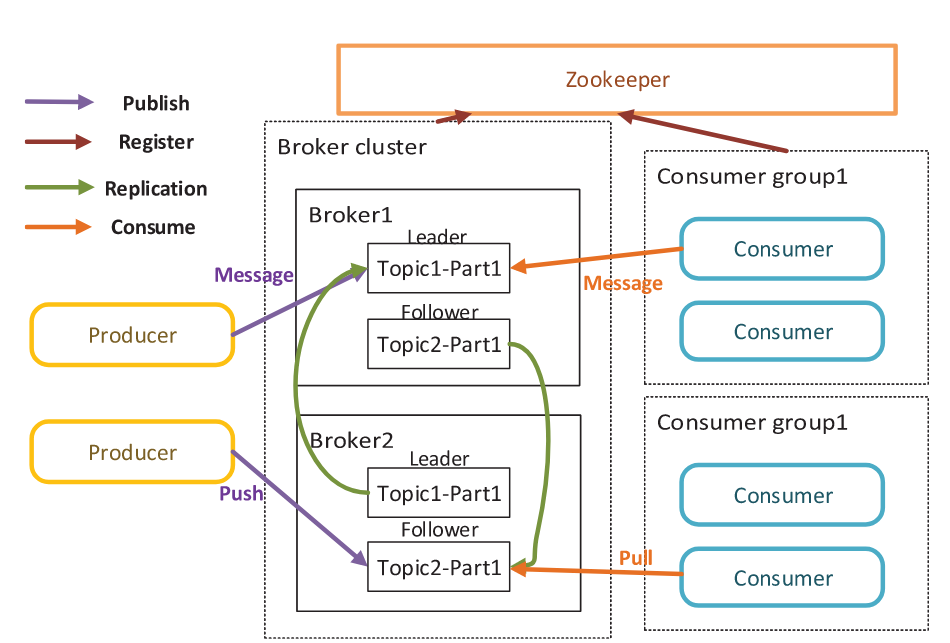
\includegraphics[width=0.8\textwidth]{content/img/Research/Message_Services/kafkaArchFairComparisonMessagingServices.png}
    \caption{Die Architektur des Apache Kafka Systems \cite{fuFairComparisonMessage2021}}
    \label{fig:kafkaArchFairComparisonMessagingServices}
\end{figure}
\FloatBarrier

Die Consumer können sich zu Gruppen zusammenschließen (\emph{Consumer-Group}) und können dadurch gemeinsam ein Topic verarbeiten. Consumer Groups können parallel mehrere Partitionen auslesen (siehe Abbildung \ref{fig:partitionsKafkaDefinitiveGuide}), jedoch werden die Messages auf die Empfänger aufgeteilt. Dadurch bieten sich Consumer-Groups perfekt für Anwendung bei \emph{Load Balancing} Use-Cases an. Außerdem benötigt Apache Kafka eine zusätzliche Applikation für das Verwalten und Koordinieren eines Clusters: \emph{Zookeeper}, zum Beispiel wird diese Applikation zur fehlerfreien und parallelen Auslesung von Topics benötigt.  \cite{narkhedeKafkaDefinitiveGuide2017}

\begin{figure}
    \centering
    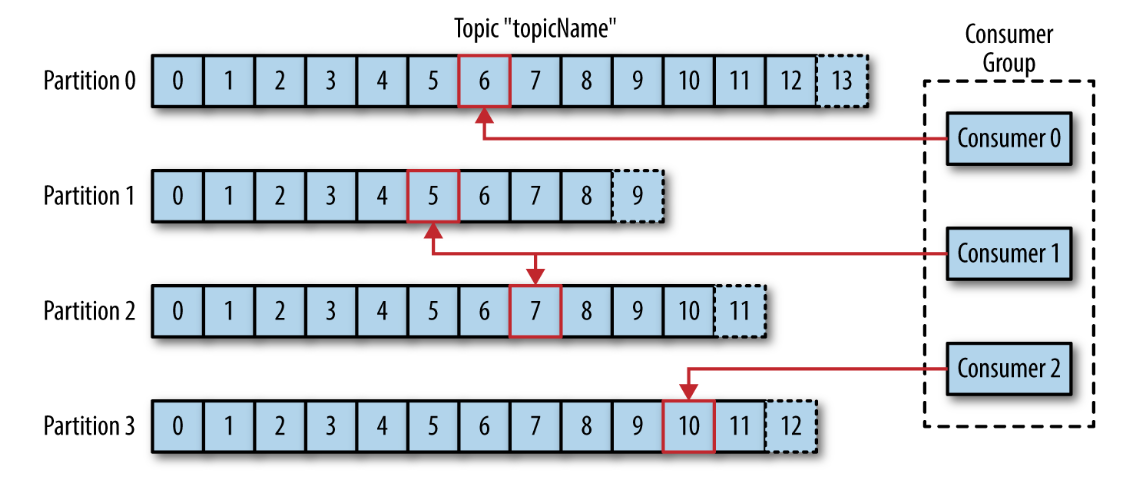
\includegraphics[width=0.8\textwidth]{content/img/Research/Message_Services/partitionsKafkaDefinitiveGuide.png}
    \caption{Eine Consumer-Group verarbeitet gemeinsam ein Topic. \cite{narkhedeKafkaDefinitiveGuide2017}}
    \label{fig:partitionsKafkaDefinitiveGuide}
\end{figure}
\FloatBarrier

Außerdem unterstützt Apache Kafka die Zustellungsgarantie At-Least-Once standardmäßig und die At-Most-Once Garantie kann bei Bedarf beim Producer eingestellt werden. Damit die Exactly-Once Zusicherung eingehalten werden kann, müssen aber Veränderungen am Ziel-Storage System bewerkstelligt werden. \cite{narkhedeKafkaDefinitiveGuide2017}

\newpage

Damit Kafka eine hohe Durchsatzrate erreicht werden kann, werden drei Methoden verwendet, die den \emph{Overhead} minimieren: \cite{narkhedeKafkaDefinitiveGuide2017}

\begin{itemize}
	\item \textbf{Die Nutzung von \emph{Zero-Copy}-Methoden}: Diese Technik wird verwendet, um Daten effizient zu übertragen, ohne dass Kopiervorgänge zwischen verschiedenen Pufferspeicherbereichen erforderlich sind. Im Kontext von Kafka wird diese Technik genutzt, um den Overhead bei der Datenübertragung zu minimieren und somit die Durchsatzraten zu verbessern.
	\item \textbf{Kafka überträgt Nachrichten in \emph{Batches}}: Durch die Stapelung von Nachrichten und deren gemeinsame Übertragung wird die Anzahl der Netzwerkverbindungen minimiert und die Effizienz der Datenübertragung gesteigert, was zu höheren Durchsatzraten führt.
	\item \textbf{Nachrichtenkomprimierung}: Diese Methode komprimiert Nachrichten, bevor sie über das Netzwerk übertragen werden, was die benötigte Netzwerkbandbreite reduziert und die Übertragungsgeschwindigkeit erhöht, was zu einer insgesamt verbesserten Durchsatzrate führt. Insbesondere wird die Leistung gesteigert, bei der Übermittlung von Nachrichten, welche gut komprimierbare Datenformate verwenden, wie zum Beispiel JSON.
\end{itemize}

Zusammenfassend lässt sich sagen, dass Apache Kafka optimal für Anwendungsfälle geeignet ist, welche eine hohe Skalierbarkeit und hohe Ausfallsicherheit benötigen. Des Weitern lässt sich Apache Kafka gut einsetzen in verteilte Systeme, welche die Anforderungen auf hohe Durchsatzraten bei der Übertragung von Nachrichten haben. Mit den Kafka Connectors ist es sogar möglich, die Anwendungsbereiche von einem Enterprise Service Bus zu decken. Jedoch ist bei der Verwendung von Kafka für Echtzeit-Kommunikation abzuraten, weil durch die Persistierung der Nachrichten auf der Festplatte Verzögerungen unvermeidbar sind. \cite{fuFairComparisonMessage2021}

\subsection{RabbitMQ}

RabbitMQ ist ein open-source Messaging Service, welcher um das Protokoll AMQP entwickelt wurde. Das System ist mit Erlang programmiert, da Erlang für das Entwickeln von verteilten Systemen geeignet ist, braucht es keine koordinierende Komponente wie Zookeeper. In der Abbildung \ref{fig:rabbitMQArchfairComparisonMessagingSystems} ist zu sehen, dass RabbitMQ auch als Cluster arbeiten kann, dafür werden die Queues auf mehrere Broker repliziert. Es gibt je Queue eine \emph{Master-Queue} und eine oder mehrere \emph{Backup-Queues}. Alle Operationen starten bei dem Master und werden zu den Backup-Queues weitergeleitet. Aber wenn die Master-Queue ausfällt, wird sofort eine Backup-Queue zur Master-Queue aufsteigen und somit ist eine hohe Ausfallsicherheit gegeben. Jedoch hat RabbitMQ kein gutes Design für Skalierbarkeit, weil die komplette Replikation der Queues nicht für hohe Auslastungen gut geeignet ist. \emph{Exchanges} sind für das \emph{Routen} der Nachrichten benötigt, sie können komplexe Routing-Anforderungen umsetzen, wie zum Beispiel die Verteilung der Nachrichten auf mehrere Queues. \cite{toshevLearningRabbitMQBuild2016}

\begin{figure}
    \centering
    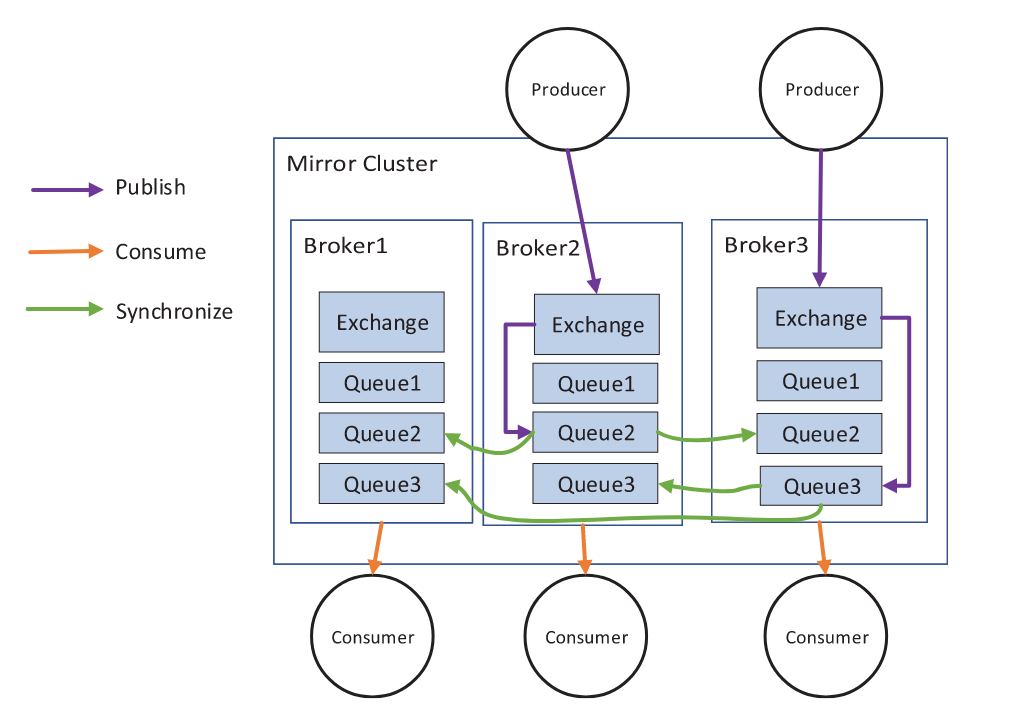
\includegraphics[width=0.9\textwidth]{content/img/Research/Message_Services/rabbitMQArchfairComparisonMessagingSystems.png}
    \caption{Die Architektur des RabbitMQ Systems \cite{fuFairComparisonMessage2021}}
    \label{fig:rabbitMQArchfairComparisonMessagingSystems}
\end{figure}
\FloatBarrier

Das RabbitMQ System ist ein general-purpose Message Broker, da es sehr viele Funktionalitäten implementiert, darunter befinden sich: \cite{toshevLearningRabbitMQBuild2016}

\begin{itemize}
	\item \textbf{Push / Pull Consumption Mode} - RabbitMQ unterstützt sowohl den Push- als auch den Pull-Konsummodus, damit kann das Messaging System perfekt an den Anwendungsfall angepasst werden.
	\item \textbf{Unterstützung von standardisierte Protokolle} - RabbitMQ unterstützt eine Vielzahl von standardisierten Protokollen, darunter AMQP (Advanced Message Queuing Protocol), MQTT (Message Queuing Telemetry Transport), STOMP (Streaming Text Oriented Messaging Protocol) und weitere. Diese Protokolle ermöglichen die Interoperabilität mit verschiedenen Clients und Systemen, was die Integration in bestehende Systeme erleichtert und die Flexibilität erhöht.
	\item \textbf{Point-to-Point und Publish-Subscribe Messaging Models} - RabbitMQ ermöglicht die Kommunikation mit dem Point-to-Point Modell oder mit dem Publish-Subscribe-Modell
	\item \textbf{Disk Nodes oder Memory Nodes für RabbitMQ Cluster} - RabbitMQ bietet die Möglichkeit, Knoten im Cluster als Disk- oder Memory-Knoten zu konfigurieren. Disk-Knoten speichern Nachrichten dauerhaft auf der Festplatte, während Memory-Knoten Nachrichten nur im Arbeitsspeicher speichern.
	\item \textbf{At-Least-Once oder At-Most-Once Zustellungsgarantien} - Durch diese Zustellungsgarantien ist die Kommunikation über RabbitMQ zuverlässig, jedoch ist die Exactly-Once Garantie von RabbitMQ nicht unterstützt. 
\end{itemize}

RabbitMQ bietet eine beeindruckende Bandbreite an Funktionalitäten, die seine Vielseitigkeit und Flexibilität unterstreichen. Diese Merkmale machen es zu einer attraktiven Option für die Integration in bestehende Systeme, da es sich nahtlos in unterschiedliche Architekturen einfügen kann. Trotz dieser Stärken steht RabbitMQ jedoch im Vergleich zu Apache Kafka in Bezug auf Skalierbarkeit und Performance zurück. Insbesondere hinsichtlich des Datendurchsatzes kann RabbitMQ nicht mit der Leistungsfähigkeit von Apache Kafka mithalten. Ein weiterer Unterschied besteht darin, dass RabbitMQ nicht die Möglichkeit bietet, Exactly-Once Semantik zu erreichen, was für bestimmte Anwendungsfälle von entscheidender Bedeutung sein kann.
\cite{toshevLearningRabbitMQBuild2016,fuFairComparisonMessage2021}

